% Created by tikzDevice version 0.9 on 2016-01-11 22:38:41
% !TEX encoding = UTF-8 Unicode
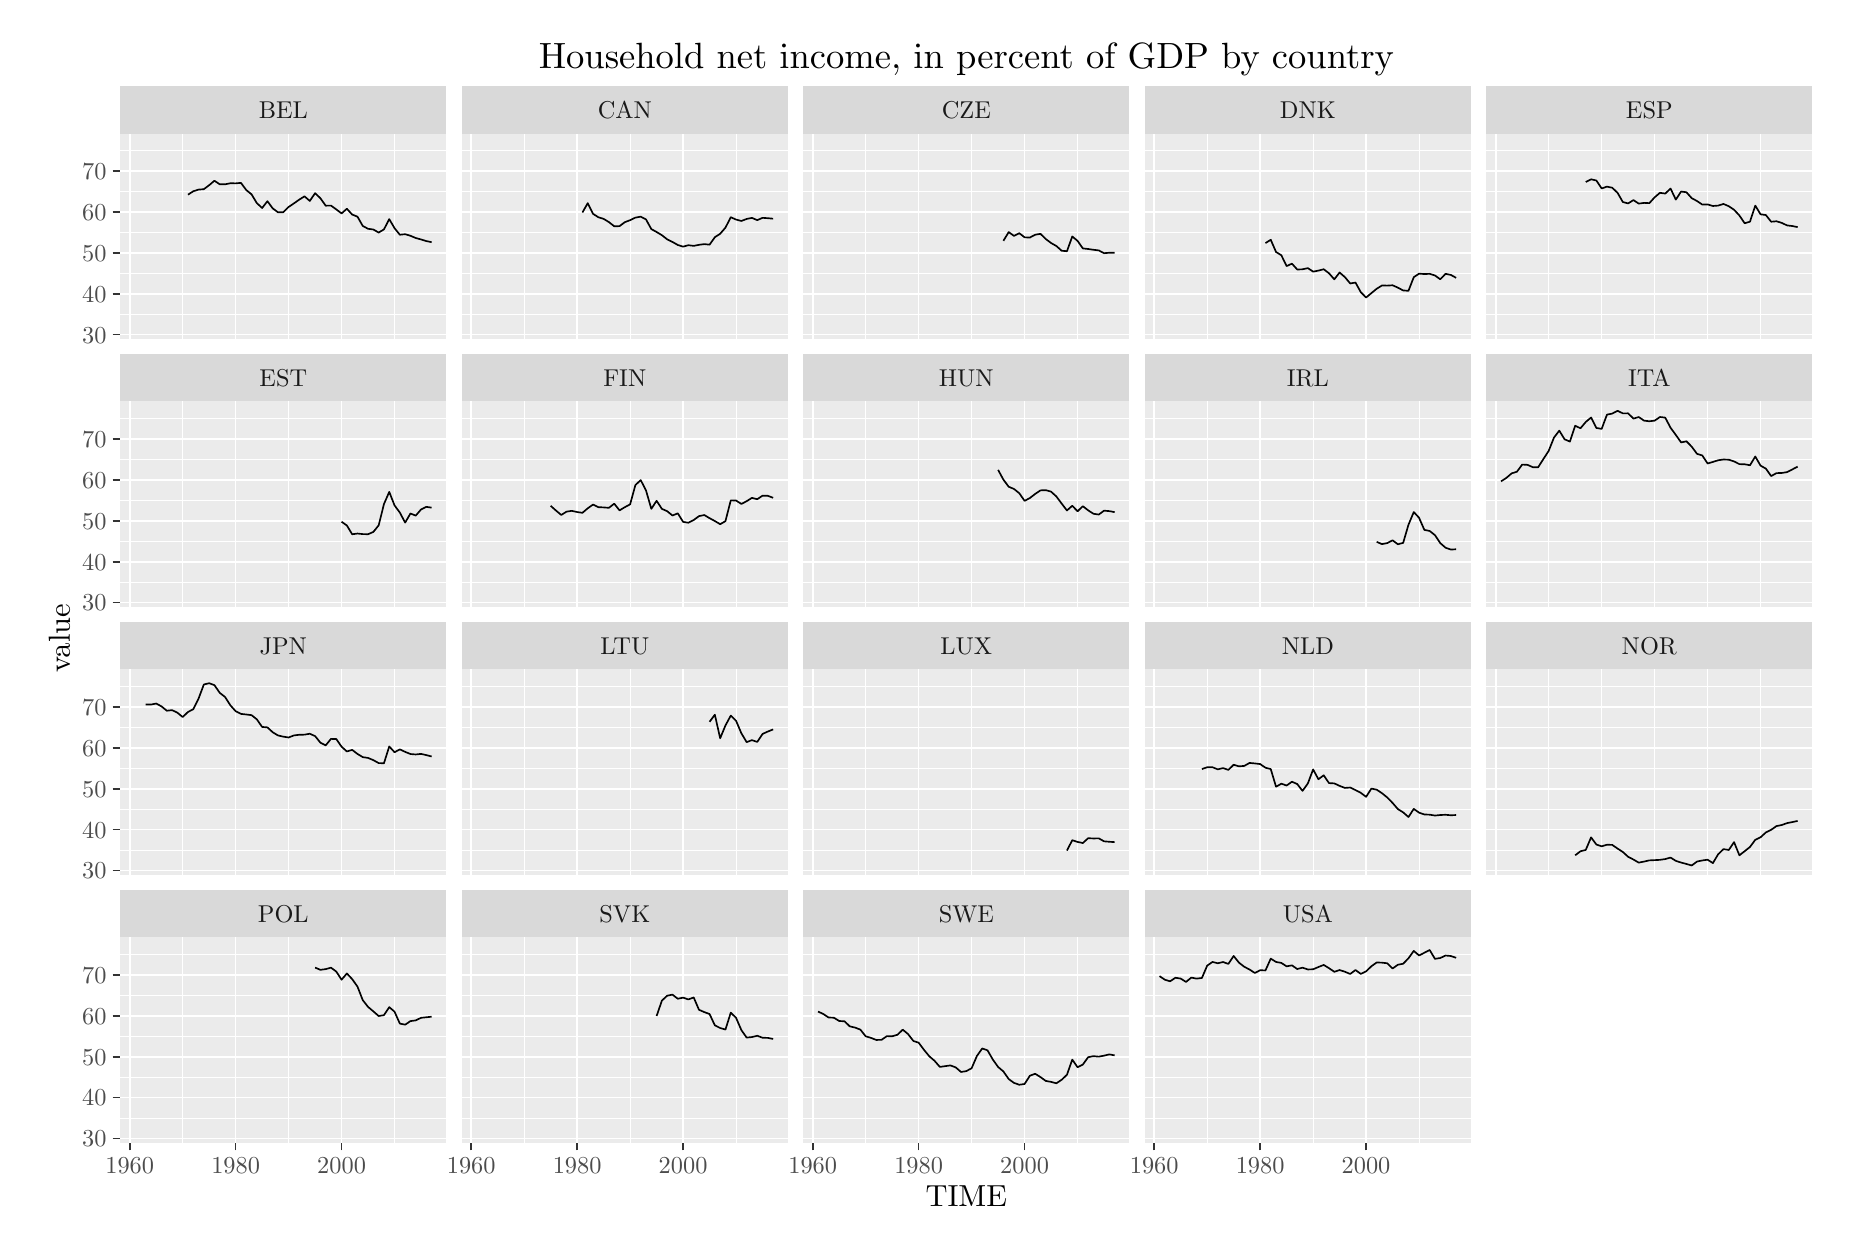
\begin{tikzpicture}[x=1pt,y=1pt]
\definecolor{fillColor}{RGB}{255,255,255}
\path[use as bounding box,fill=fillColor,fill opacity=0.00] (0,0) rectangle (650.43,433.62);
\begin{scope}
\path[clip] (  0.00,  0.00) rectangle (650.43,433.62);
\definecolor{drawColor}{RGB}{255,255,255}
\definecolor{fillColor}{RGB}{255,255,255}

\path[draw=drawColor,line width= 0.6pt,line join=round,line cap=round,fill=fillColor] (  0.00,  0.00) rectangle (650.43,433.62);
\end{scope}
\begin{scope}
\path[clip] ( 33.42,321.12) rectangle (151.33,395.37);
\definecolor{fillColor}{gray}{0.92}

\path[fill=fillColor] ( 33.42,321.12) rectangle (151.33,395.37);
\definecolor{drawColor}{RGB}{255,255,255}

\path[draw=drawColor,line width= 0.3pt,line join=round] ( 33.42,330.07) --
	(151.33,330.07);

\path[draw=drawColor,line width= 0.3pt,line join=round] ( 33.42,344.83) --
	(151.33,344.83);

\path[draw=drawColor,line width= 0.3pt,line join=round] ( 33.42,359.60) --
	(151.33,359.60);

\path[draw=drawColor,line width= 0.3pt,line join=round] ( 33.42,374.36) --
	(151.33,374.36);

\path[draw=drawColor,line width= 0.3pt,line join=round] ( 33.42,389.12) --
	(151.33,389.12);

\path[draw=drawColor,line width= 0.3pt,line join=round] ( 56.01,321.12) --
	( 56.01,395.37);

\path[draw=drawColor,line width= 0.3pt,line join=round] ( 94.29,321.12) --
	( 94.29,395.37);

\path[draw=drawColor,line width= 0.3pt,line join=round] (132.57,321.12) --
	(132.57,395.37);

\path[draw=drawColor,line width= 0.6pt,line join=round] ( 33.42,322.69) --
	(151.33,322.69);

\path[draw=drawColor,line width= 0.6pt,line join=round] ( 33.42,337.45) --
	(151.33,337.45);

\path[draw=drawColor,line width= 0.6pt,line join=round] ( 33.42,352.21) --
	(151.33,352.21);

\path[draw=drawColor,line width= 0.6pt,line join=round] ( 33.42,366.98) --
	(151.33,366.98);

\path[draw=drawColor,line width= 0.6pt,line join=round] ( 33.42,381.74) --
	(151.33,381.74);

\path[draw=drawColor,line width= 0.6pt,line join=round] ( 36.87,321.12) --
	( 36.87,395.37);

\path[draw=drawColor,line width= 0.6pt,line join=round] ( 75.15,321.12) --
	( 75.15,395.37);

\path[draw=drawColor,line width= 0.6pt,line join=round] (113.43,321.12) --
	(113.43,395.37);
\definecolor{drawColor}{RGB}{0,0,0}

\path[draw=drawColor,line width= 0.6pt,line join=round] ( 57.92,373.27) --
	( 59.84,374.50) --
	( 61.75,375.11) --
	( 63.66,375.25) --
	( 65.58,376.70) --
	( 67.49,378.31) --
	( 69.41,377.03) --
	( 71.32,377.01) --
	( 73.23,377.39) --
	( 75.15,377.36) --
	( 77.06,377.54) --
	( 78.98,374.95) --
	( 80.89,373.39) --
	( 82.80,370.23) --
	( 84.72,368.46) --
	( 86.63,370.91) --
	( 88.55,368.31) --
	( 90.46,366.89) --
	( 92.37,366.93) --
	( 94.29,368.83) --
	( 96.20,370.12) --
	( 98.12,371.47) --
	(100.03,372.67) --
	(101.94,371.00) --
	(103.86,373.81) --
	(105.77,371.98) --
	(107.69,369.29) --
	(109.60,369.32) --
	(111.51,367.95) --
	(113.43,366.49) --
	(115.34,368.18) --
	(117.26,366.08) --
	(119.17,365.32) --
	(121.08,361.97) --
	(123.00,360.94) --
	(124.91,360.69) --
	(126.83,359.58) --
	(128.74,360.72) --
	(130.65,364.44) --
	(132.57,361.16) --
	(134.48,358.79) --
	(136.40,358.99) --
	(138.31,358.42) --
	(140.22,357.61) --
	(142.14,357.09) --
	(144.05,356.50) --
	(145.97,356.10);
\end{scope}
\begin{scope}
\path[clip] (156.83,321.12) rectangle (274.73,395.37);
\definecolor{fillColor}{gray}{0.92}

\path[fill=fillColor] (156.83,321.12) rectangle (274.73,395.37);
\definecolor{drawColor}{RGB}{255,255,255}

\path[draw=drawColor,line width= 0.3pt,line join=round] (156.83,330.07) --
	(274.73,330.07);

\path[draw=drawColor,line width= 0.3pt,line join=round] (156.83,344.83) --
	(274.73,344.83);

\path[draw=drawColor,line width= 0.3pt,line join=round] (156.83,359.60) --
	(274.73,359.60);

\path[draw=drawColor,line width= 0.3pt,line join=round] (156.83,374.36) --
	(274.73,374.36);

\path[draw=drawColor,line width= 0.3pt,line join=round] (156.83,389.12) --
	(274.73,389.12);

\path[draw=drawColor,line width= 0.3pt,line join=round] (179.41,321.12) --
	(179.41,395.37);

\path[draw=drawColor,line width= 0.3pt,line join=round] (217.69,321.12) --
	(217.69,395.37);

\path[draw=drawColor,line width= 0.3pt,line join=round] (255.97,321.12) --
	(255.97,395.37);

\path[draw=drawColor,line width= 0.6pt,line join=round] (156.83,322.69) --
	(274.73,322.69);

\path[draw=drawColor,line width= 0.6pt,line join=round] (156.83,337.45) --
	(274.73,337.45);

\path[draw=drawColor,line width= 0.6pt,line join=round] (156.83,352.21) --
	(274.73,352.21);

\path[draw=drawColor,line width= 0.6pt,line join=round] (156.83,366.98) --
	(274.73,366.98);

\path[draw=drawColor,line width= 0.6pt,line join=round] (156.83,381.74) --
	(274.73,381.74);

\path[draw=drawColor,line width= 0.6pt,line join=round] (160.27,321.12) --
	(160.27,395.37);

\path[draw=drawColor,line width= 0.6pt,line join=round] (198.55,321.12) --
	(198.55,395.37);

\path[draw=drawColor,line width= 0.6pt,line join=round] (236.83,321.12) --
	(236.83,395.37);
\definecolor{drawColor}{RGB}{0,0,0}

\path[draw=drawColor,line width= 0.6pt,line join=round] (200.46,366.83) --
	(202.38,370.21) --
	(204.29,366.35) --
	(206.21,365.11) --
	(208.12,364.53) --
	(210.03,363.36) --
	(211.95,361.85) --
	(213.86,361.90) --
	(215.78,363.34) --
	(217.69,364.05) --
	(219.60,364.98) --
	(221.52,365.33) --
	(223.43,364.32) --
	(225.35,360.84) --
	(227.26,359.78) --
	(229.17,358.62) --
	(231.09,357.13) --
	(233.00,356.19) --
	(234.92,355.09) --
	(236.83,354.49) --
	(238.74,355.01) --
	(240.66,354.77) --
	(242.57,355.15) --
	(244.49,355.40) --
	(246.40,355.20) --
	(248.31,357.89) --
	(250.23,359.15) --
	(252.14,361.35) --
	(254.06,365.13) --
	(255.97,364.27) --
	(257.88,363.77) --
	(259.80,364.49) --
	(261.71,364.89) --
	(263.63,364.06) --
	(265.54,364.90) --
	(267.45,364.77) --
	(269.37,364.59);
\end{scope}
\begin{scope}
\path[clip] (280.23,321.12) rectangle (398.13,395.37);
\definecolor{fillColor}{gray}{0.92}

\path[fill=fillColor] (280.23,321.12) rectangle (398.13,395.37);
\definecolor{drawColor}{RGB}{255,255,255}

\path[draw=drawColor,line width= 0.3pt,line join=round] (280.23,330.07) --
	(398.13,330.07);

\path[draw=drawColor,line width= 0.3pt,line join=round] (280.23,344.83) --
	(398.13,344.83);

\path[draw=drawColor,line width= 0.3pt,line join=round] (280.23,359.60) --
	(398.13,359.60);

\path[draw=drawColor,line width= 0.3pt,line join=round] (280.23,374.36) --
	(398.13,374.36);

\path[draw=drawColor,line width= 0.3pt,line join=round] (280.23,389.12) --
	(398.13,389.12);

\path[draw=drawColor,line width= 0.3pt,line join=round] (302.81,321.12) --
	(302.81,395.37);

\path[draw=drawColor,line width= 0.3pt,line join=round] (341.09,321.12) --
	(341.09,395.37);

\path[draw=drawColor,line width= 0.3pt,line join=round] (379.37,321.12) --
	(379.37,395.37);

\path[draw=drawColor,line width= 0.6pt,line join=round] (280.23,322.69) --
	(398.13,322.69);

\path[draw=drawColor,line width= 0.6pt,line join=round] (280.23,337.45) --
	(398.13,337.45);

\path[draw=drawColor,line width= 0.6pt,line join=round] (280.23,352.21) --
	(398.13,352.21);

\path[draw=drawColor,line width= 0.6pt,line join=round] (280.23,366.98) --
	(398.13,366.98);

\path[draw=drawColor,line width= 0.6pt,line join=round] (280.23,381.74) --
	(398.13,381.74);

\path[draw=drawColor,line width= 0.6pt,line join=round] (283.67,321.12) --
	(283.67,395.37);

\path[draw=drawColor,line width= 0.6pt,line join=round] (321.95,321.12) --
	(321.95,395.37);

\path[draw=drawColor,line width= 0.6pt,line join=round] (360.23,321.12) --
	(360.23,395.37);
\definecolor{drawColor}{RGB}{0,0,0}

\path[draw=drawColor,line width= 0.6pt,line join=round] (352.57,356.59) --
	(354.49,359.75) --
	(356.40,358.37) --
	(358.32,359.36) --
	(360.23,357.85) --
	(362.14,357.78) --
	(364.06,358.80) --
	(365.97,359.12) --
	(367.89,357.24) --
	(369.80,355.80) --
	(371.71,354.72) --
	(373.63,353.01) --
	(375.54,352.84) --
	(377.46,358.16) --
	(379.37,356.58) --
	(381.28,353.85) --
	(383.20,353.64) --
	(385.11,353.36) --
	(387.03,353.13) --
	(388.94,352.12) --
	(390.85,352.28) --
	(392.77,352.26);
\end{scope}
\begin{scope}
\path[clip] (403.63,321.12) rectangle (521.53,395.37);
\definecolor{fillColor}{gray}{0.92}

\path[fill=fillColor] (403.63,321.12) rectangle (521.53,395.37);
\definecolor{drawColor}{RGB}{255,255,255}

\path[draw=drawColor,line width= 0.3pt,line join=round] (403.63,330.07) --
	(521.53,330.07);

\path[draw=drawColor,line width= 0.3pt,line join=round] (403.63,344.83) --
	(521.53,344.83);

\path[draw=drawColor,line width= 0.3pt,line join=round] (403.63,359.60) --
	(521.53,359.60);

\path[draw=drawColor,line width= 0.3pt,line join=round] (403.63,374.36) --
	(521.53,374.36);

\path[draw=drawColor,line width= 0.3pt,line join=round] (403.63,389.12) --
	(521.53,389.12);

\path[draw=drawColor,line width= 0.3pt,line join=round] (426.21,321.12) --
	(426.21,395.37);

\path[draw=drawColor,line width= 0.3pt,line join=round] (464.49,321.12) --
	(464.49,395.37);

\path[draw=drawColor,line width= 0.3pt,line join=round] (502.77,321.12) --
	(502.77,395.37);

\path[draw=drawColor,line width= 0.6pt,line join=round] (403.63,322.69) --
	(521.53,322.69);

\path[draw=drawColor,line width= 0.6pt,line join=round] (403.63,337.45) --
	(521.53,337.45);

\path[draw=drawColor,line width= 0.6pt,line join=round] (403.63,352.21) --
	(521.53,352.21);

\path[draw=drawColor,line width= 0.6pt,line join=round] (403.63,366.98) --
	(521.53,366.98);

\path[draw=drawColor,line width= 0.6pt,line join=round] (403.63,381.74) --
	(521.53,381.74);

\path[draw=drawColor,line width= 0.6pt,line join=round] (407.07,321.12) --
	(407.07,395.37);

\path[draw=drawColor,line width= 0.6pt,line join=round] (445.35,321.12) --
	(445.35,395.37);

\path[draw=drawColor,line width= 0.6pt,line join=round] (483.63,321.12) --
	(483.63,395.37);
\definecolor{drawColor}{RGB}{0,0,0}

\path[draw=drawColor,line width= 0.6pt,line join=round] (447.27,355.78) --
	(449.18,356.97) --
	(451.09,352.56) --
	(453.01,351.37) --
	(454.92,347.46) --
	(456.84,348.35) --
	(458.75,346.23) --
	(460.66,346.30) --
	(462.58,346.73) --
	(464.49,345.45) --
	(466.41,345.83) --
	(468.32,346.33) --
	(470.23,344.86) --
	(472.15,342.68) --
	(474.06,345.15) --
	(475.98,343.47) --
	(477.89,341.18) --
	(479.80,341.52) --
	(481.72,338.04) --
	(483.63,336.10) --
	(485.55,337.70) --
	(487.46,339.27) --
	(489.37,340.46) --
	(491.29,340.41) --
	(493.20,340.53) --
	(495.12,339.67) --
	(497.03,338.66) --
	(498.94,338.53) --
	(500.86,343.45) --
	(502.77,344.72) --
	(504.69,344.59) --
	(506.60,344.67) --
	(508.51,344.07) --
	(510.43,342.70) --
	(512.34,344.66) --
	(514.26,344.27) --
	(516.17,343.22);
\end{scope}
\begin{scope}
\path[clip] (527.03,321.12) rectangle (644.93,395.37);
\definecolor{fillColor}{gray}{0.92}

\path[fill=fillColor] (527.03,321.12) rectangle (644.93,395.37);
\definecolor{drawColor}{RGB}{255,255,255}

\path[draw=drawColor,line width= 0.3pt,line join=round] (527.03,330.07) --
	(644.93,330.07);

\path[draw=drawColor,line width= 0.3pt,line join=round] (527.03,344.83) --
	(644.93,344.83);

\path[draw=drawColor,line width= 0.3pt,line join=round] (527.03,359.60) --
	(644.93,359.60);

\path[draw=drawColor,line width= 0.3pt,line join=round] (527.03,374.36) --
	(644.93,374.36);

\path[draw=drawColor,line width= 0.3pt,line join=round] (527.03,389.12) --
	(644.93,389.12);

\path[draw=drawColor,line width= 0.3pt,line join=round] (549.61,321.12) --
	(549.61,395.37);

\path[draw=drawColor,line width= 0.3pt,line join=round] (587.89,321.12) --
	(587.89,395.37);

\path[draw=drawColor,line width= 0.3pt,line join=round] (626.17,321.12) --
	(626.17,395.37);

\path[draw=drawColor,line width= 0.6pt,line join=round] (527.03,322.69) --
	(644.93,322.69);

\path[draw=drawColor,line width= 0.6pt,line join=round] (527.03,337.45) --
	(644.93,337.45);

\path[draw=drawColor,line width= 0.6pt,line join=round] (527.03,352.21) --
	(644.93,352.21);

\path[draw=drawColor,line width= 0.6pt,line join=round] (527.03,366.98) --
	(644.93,366.98);

\path[draw=drawColor,line width= 0.6pt,line join=round] (527.03,381.74) --
	(644.93,381.74);

\path[draw=drawColor,line width= 0.6pt,line join=round] (530.47,321.12) --
	(530.47,395.37);

\path[draw=drawColor,line width= 0.6pt,line join=round] (568.75,321.12) --
	(568.75,395.37);

\path[draw=drawColor,line width= 0.6pt,line join=round] (607.03,321.12) --
	(607.03,395.37);
\definecolor{drawColor}{RGB}{0,0,0}

\path[draw=drawColor,line width= 0.6pt,line join=round] (563.01,377.84) --
	(564.93,378.83) --
	(566.84,378.38) --
	(568.75,375.52) --
	(570.67,376.18) --
	(572.58,375.77) --
	(574.50,373.93) --
	(576.41,370.61) --
	(578.32,370.11) --
	(580.24,371.32) --
	(582.15,370.04) --
	(584.07,370.30) --
	(585.98,370.21) --
	(587.89,372.30) --
	(589.81,373.95) --
	(591.72,373.66) --
	(593.64,375.49) --
	(595.55,371.49) --
	(597.46,374.40) --
	(599.38,374.15) --
	(601.29,372.01) --
	(603.21,370.98) --
	(605.12,369.68) --
	(607.03,369.75) --
	(608.95,369.18) --
	(610.86,369.33) --
	(612.78,369.92) --
	(614.69,369.10) --
	(616.60,367.82) --
	(618.52,365.75) --
	(620.43,362.94) --
	(622.35,363.51) --
	(624.26,369.33) --
	(626.17,366.17) --
	(628.09,365.91) --
	(630.00,363.49) --
	(631.91,363.66) --
	(633.83,363.08) --
	(635.74,362.16) --
	(637.66,361.94) --
	(639.57,361.55);
\end{scope}
\begin{scope}
\path[clip] ( 33.42,224.31) rectangle (151.33,298.56);
\definecolor{fillColor}{gray}{0.92}

\path[fill=fillColor] ( 33.42,224.31) rectangle (151.33,298.56);
\definecolor{drawColor}{RGB}{255,255,255}

\path[draw=drawColor,line width= 0.3pt,line join=round] ( 33.42,233.26) --
	(151.33,233.26);

\path[draw=drawColor,line width= 0.3pt,line join=round] ( 33.42,248.02) --
	(151.33,248.02);

\path[draw=drawColor,line width= 0.3pt,line join=round] ( 33.42,262.79) --
	(151.33,262.79);

\path[draw=drawColor,line width= 0.3pt,line join=round] ( 33.42,277.55) --
	(151.33,277.55);

\path[draw=drawColor,line width= 0.3pt,line join=round] ( 33.42,292.31) --
	(151.33,292.31);

\path[draw=drawColor,line width= 0.3pt,line join=round] ( 56.01,224.31) --
	( 56.01,298.56);

\path[draw=drawColor,line width= 0.3pt,line join=round] ( 94.29,224.31) --
	( 94.29,298.56);

\path[draw=drawColor,line width= 0.3pt,line join=round] (132.57,224.31) --
	(132.57,298.56);

\path[draw=drawColor,line width= 0.6pt,line join=round] ( 33.42,225.88) --
	(151.33,225.88);

\path[draw=drawColor,line width= 0.6pt,line join=round] ( 33.42,240.64) --
	(151.33,240.64);

\path[draw=drawColor,line width= 0.6pt,line join=round] ( 33.42,255.40) --
	(151.33,255.40);

\path[draw=drawColor,line width= 0.6pt,line join=round] ( 33.42,270.17) --
	(151.33,270.17);

\path[draw=drawColor,line width= 0.6pt,line join=round] ( 33.42,284.93) --
	(151.33,284.93);

\path[draw=drawColor,line width= 0.6pt,line join=round] ( 36.87,224.31) --
	( 36.87,298.56);

\path[draw=drawColor,line width= 0.6pt,line join=round] ( 75.15,224.31) --
	( 75.15,298.56);

\path[draw=drawColor,line width= 0.6pt,line join=round] (113.43,224.31) --
	(113.43,298.56);
\definecolor{drawColor}{RGB}{0,0,0}

\path[draw=drawColor,line width= 0.6pt,line join=round] (113.43,255.08) --
	(115.34,253.73) --
	(117.26,250.56) --
	(119.17,250.82) --
	(121.08,250.62) --
	(123.00,250.57) --
	(124.91,251.41) --
	(126.83,253.78) --
	(128.74,261.47) --
	(130.65,265.87) --
	(132.57,260.98) --
	(134.48,258.40) --
	(136.40,254.77) --
	(138.31,258.06) --
	(140.22,257.29) --
	(142.14,259.53) --
	(144.05,260.47) --
	(145.97,260.17);
\end{scope}
\begin{scope}
\path[clip] (156.83,224.31) rectangle (274.73,298.56);
\definecolor{fillColor}{gray}{0.92}

\path[fill=fillColor] (156.83,224.31) rectangle (274.73,298.56);
\definecolor{drawColor}{RGB}{255,255,255}

\path[draw=drawColor,line width= 0.3pt,line join=round] (156.83,233.26) --
	(274.73,233.26);

\path[draw=drawColor,line width= 0.3pt,line join=round] (156.83,248.02) --
	(274.73,248.02);

\path[draw=drawColor,line width= 0.3pt,line join=round] (156.83,262.79) --
	(274.73,262.79);

\path[draw=drawColor,line width= 0.3pt,line join=round] (156.83,277.55) --
	(274.73,277.55);

\path[draw=drawColor,line width= 0.3pt,line join=round] (156.83,292.31) --
	(274.73,292.31);

\path[draw=drawColor,line width= 0.3pt,line join=round] (179.41,224.31) --
	(179.41,298.56);

\path[draw=drawColor,line width= 0.3pt,line join=round] (217.69,224.31) --
	(217.69,298.56);

\path[draw=drawColor,line width= 0.3pt,line join=round] (255.97,224.31) --
	(255.97,298.56);

\path[draw=drawColor,line width= 0.6pt,line join=round] (156.83,225.88) --
	(274.73,225.88);

\path[draw=drawColor,line width= 0.6pt,line join=round] (156.83,240.64) --
	(274.73,240.64);

\path[draw=drawColor,line width= 0.6pt,line join=round] (156.83,255.40) --
	(274.73,255.40);

\path[draw=drawColor,line width= 0.6pt,line join=round] (156.83,270.17) --
	(274.73,270.17);

\path[draw=drawColor,line width= 0.6pt,line join=round] (156.83,284.93) --
	(274.73,284.93);

\path[draw=drawColor,line width= 0.6pt,line join=round] (160.27,224.31) --
	(160.27,298.56);

\path[draw=drawColor,line width= 0.6pt,line join=round] (198.55,224.31) --
	(198.55,298.56);

\path[draw=drawColor,line width= 0.6pt,line join=round] (236.83,224.31) --
	(236.83,298.56);
\definecolor{drawColor}{RGB}{0,0,0}

\path[draw=drawColor,line width= 0.6pt,line join=round] (188.98,260.83) --
	(190.89,259.14) --
	(192.81,257.53) --
	(194.72,258.74) --
	(196.64,259.02) --
	(198.55,258.59) --
	(200.46,258.31) --
	(202.38,259.94) --
	(204.29,261.29) --
	(206.21,260.35) --
	(208.12,260.26) --
	(210.03,260.11) --
	(211.95,261.62) --
	(213.86,259.19) --
	(215.78,260.35) --
	(217.69,261.37) --
	(219.60,268.35) --
	(221.52,270.13) --
	(223.43,266.40) --
	(225.35,259.75) --
	(227.26,262.65) --
	(229.17,259.74) --
	(231.09,258.89) --
	(233.00,257.33) --
	(234.92,258.13) --
	(236.83,255.04) --
	(238.74,254.72) --
	(240.66,255.70) --
	(242.57,257.11) --
	(244.49,257.51) --
	(246.40,256.37) --
	(248.31,255.34) --
	(250.23,254.19) --
	(252.14,255.30) --
	(254.06,262.80) --
	(255.97,262.77) --
	(257.88,261.51) --
	(259.80,262.51) --
	(261.71,263.71) --
	(263.63,263.22) --
	(265.54,264.49) --
	(267.45,264.46) --
	(269.37,263.73);
\end{scope}
\begin{scope}
\path[clip] (280.23,224.31) rectangle (398.13,298.56);
\definecolor{fillColor}{gray}{0.92}

\path[fill=fillColor] (280.23,224.31) rectangle (398.13,298.56);
\definecolor{drawColor}{RGB}{255,255,255}

\path[draw=drawColor,line width= 0.3pt,line join=round] (280.23,233.26) --
	(398.13,233.26);

\path[draw=drawColor,line width= 0.3pt,line join=round] (280.23,248.02) --
	(398.13,248.02);

\path[draw=drawColor,line width= 0.3pt,line join=round] (280.23,262.79) --
	(398.13,262.79);

\path[draw=drawColor,line width= 0.3pt,line join=round] (280.23,277.55) --
	(398.13,277.55);

\path[draw=drawColor,line width= 0.3pt,line join=round] (280.23,292.31) --
	(398.13,292.31);

\path[draw=drawColor,line width= 0.3pt,line join=round] (302.81,224.31) --
	(302.81,298.56);

\path[draw=drawColor,line width= 0.3pt,line join=round] (341.09,224.31) --
	(341.09,298.56);

\path[draw=drawColor,line width= 0.3pt,line join=round] (379.37,224.31) --
	(379.37,298.56);

\path[draw=drawColor,line width= 0.6pt,line join=round] (280.23,225.88) --
	(398.13,225.88);

\path[draw=drawColor,line width= 0.6pt,line join=round] (280.23,240.64) --
	(398.13,240.64);

\path[draw=drawColor,line width= 0.6pt,line join=round] (280.23,255.40) --
	(398.13,255.40);

\path[draw=drawColor,line width= 0.6pt,line join=round] (280.23,270.17) --
	(398.13,270.17);

\path[draw=drawColor,line width= 0.6pt,line join=round] (280.23,284.93) --
	(398.13,284.93);

\path[draw=drawColor,line width= 0.6pt,line join=round] (283.67,224.31) --
	(283.67,298.56);

\path[draw=drawColor,line width= 0.6pt,line join=round] (321.95,224.31) --
	(321.95,298.56);

\path[draw=drawColor,line width= 0.6pt,line join=round] (360.23,224.31) --
	(360.23,298.56);
\definecolor{drawColor}{RGB}{0,0,0}

\path[draw=drawColor,line width= 0.6pt,line join=round] (350.66,273.83) --
	(352.57,270.30) --
	(354.49,267.73) --
	(356.40,266.93) --
	(358.32,265.38) --
	(360.23,262.63) --
	(362.14,263.66) --
	(364.06,265.13) --
	(365.97,266.42) --
	(367.89,266.50) --
	(369.80,265.96) --
	(371.71,264.22) --
	(373.63,261.64) --
	(375.54,259.16) --
	(377.46,260.87) --
	(379.37,258.87) --
	(381.28,260.70) --
	(383.20,259.21) --
	(385.11,257.97) --
	(387.03,257.68) --
	(388.94,259.08) --
	(390.85,258.92) --
	(392.77,258.55);
\end{scope}
\begin{scope}
\path[clip] (403.63,224.31) rectangle (521.53,298.56);
\definecolor{fillColor}{gray}{0.92}

\path[fill=fillColor] (403.63,224.31) rectangle (521.53,298.56);
\definecolor{drawColor}{RGB}{255,255,255}

\path[draw=drawColor,line width= 0.3pt,line join=round] (403.63,233.26) --
	(521.53,233.26);

\path[draw=drawColor,line width= 0.3pt,line join=round] (403.63,248.02) --
	(521.53,248.02);

\path[draw=drawColor,line width= 0.3pt,line join=round] (403.63,262.79) --
	(521.53,262.79);

\path[draw=drawColor,line width= 0.3pt,line join=round] (403.63,277.55) --
	(521.53,277.55);

\path[draw=drawColor,line width= 0.3pt,line join=round] (403.63,292.31) --
	(521.53,292.31);

\path[draw=drawColor,line width= 0.3pt,line join=round] (426.21,224.31) --
	(426.21,298.56);

\path[draw=drawColor,line width= 0.3pt,line join=round] (464.49,224.31) --
	(464.49,298.56);

\path[draw=drawColor,line width= 0.3pt,line join=round] (502.77,224.31) --
	(502.77,298.56);

\path[draw=drawColor,line width= 0.6pt,line join=round] (403.63,225.88) --
	(521.53,225.88);

\path[draw=drawColor,line width= 0.6pt,line join=round] (403.63,240.64) --
	(521.53,240.64);

\path[draw=drawColor,line width= 0.6pt,line join=round] (403.63,255.40) --
	(521.53,255.40);

\path[draw=drawColor,line width= 0.6pt,line join=round] (403.63,270.17) --
	(521.53,270.17);

\path[draw=drawColor,line width= 0.6pt,line join=round] (403.63,284.93) --
	(521.53,284.93);

\path[draw=drawColor,line width= 0.6pt,line join=round] (407.07,224.31) --
	(407.07,298.56);

\path[draw=drawColor,line width= 0.6pt,line join=round] (445.35,224.31) --
	(445.35,298.56);

\path[draw=drawColor,line width= 0.6pt,line join=round] (483.63,224.31) --
	(483.63,298.56);
\definecolor{drawColor}{RGB}{0,0,0}

\path[draw=drawColor,line width= 0.6pt,line join=round] (487.46,247.82) --
	(489.37,246.99) --
	(491.29,247.38) --
	(493.20,248.37) --
	(495.12,246.94) --
	(497.03,247.46) --
	(498.94,253.99) --
	(500.86,258.59) --
	(502.77,256.53) --
	(504.69,252.13) --
	(506.60,251.76) --
	(508.51,250.24) --
	(510.43,247.37) --
	(512.34,245.70) --
	(514.26,245.03) --
	(516.17,245.14);
\end{scope}
\begin{scope}
\path[clip] (527.03,224.31) rectangle (644.93,298.56);
\definecolor{fillColor}{gray}{0.92}

\path[fill=fillColor] (527.03,224.31) rectangle (644.93,298.56);
\definecolor{drawColor}{RGB}{255,255,255}

\path[draw=drawColor,line width= 0.3pt,line join=round] (527.03,233.26) --
	(644.93,233.26);

\path[draw=drawColor,line width= 0.3pt,line join=round] (527.03,248.02) --
	(644.93,248.02);

\path[draw=drawColor,line width= 0.3pt,line join=round] (527.03,262.79) --
	(644.93,262.79);

\path[draw=drawColor,line width= 0.3pt,line join=round] (527.03,277.55) --
	(644.93,277.55);

\path[draw=drawColor,line width= 0.3pt,line join=round] (527.03,292.31) --
	(644.93,292.31);

\path[draw=drawColor,line width= 0.3pt,line join=round] (549.61,224.31) --
	(549.61,298.56);

\path[draw=drawColor,line width= 0.3pt,line join=round] (587.89,224.31) --
	(587.89,298.56);

\path[draw=drawColor,line width= 0.3pt,line join=round] (626.17,224.31) --
	(626.17,298.56);

\path[draw=drawColor,line width= 0.6pt,line join=round] (527.03,225.88) --
	(644.93,225.88);

\path[draw=drawColor,line width= 0.6pt,line join=round] (527.03,240.64) --
	(644.93,240.64);

\path[draw=drawColor,line width= 0.6pt,line join=round] (527.03,255.40) --
	(644.93,255.40);

\path[draw=drawColor,line width= 0.6pt,line join=round] (527.03,270.17) --
	(644.93,270.17);

\path[draw=drawColor,line width= 0.6pt,line join=round] (527.03,284.93) --
	(644.93,284.93);

\path[draw=drawColor,line width= 0.6pt,line join=round] (530.47,224.31) --
	(530.47,298.56);

\path[draw=drawColor,line width= 0.6pt,line join=round] (568.75,224.31) --
	(568.75,298.56);

\path[draw=drawColor,line width= 0.6pt,line join=round] (607.03,224.31) --
	(607.03,298.56);
\definecolor{drawColor}{RGB}{0,0,0}

\path[draw=drawColor,line width= 0.6pt,line join=round] (532.39,269.68) --
	(534.30,270.91) --
	(536.22,272.56) --
	(538.13,273.15) --
	(540.04,275.74) --
	(541.96,275.64) --
	(543.87,274.80) --
	(545.79,274.76) --
	(547.70,277.75) --
	(549.61,280.69) --
	(551.53,285.51) --
	(553.44,288.00) --
	(555.36,284.87) --
	(557.27,284.06) --
	(559.18,289.77) --
	(561.10,288.86) --
	(563.01,291.13) --
	(564.93,292.75) --
	(566.84,288.98) --
	(568.75,288.63) --
	(570.67,293.78) --
	(572.58,294.17) --
	(574.50,295.18) --
	(576.41,294.25) --
	(578.32,294.26) --
	(580.24,292.35) --
	(582.15,292.92) --
	(584.07,291.62) --
	(585.98,291.39) --
	(587.89,291.61) --
	(589.81,292.93) --
	(591.72,292.71) --
	(593.64,289.06) --
	(595.55,286.46) --
	(597.46,283.74) --
	(599.38,284.15) --
	(601.29,282.22) --
	(603.21,279.62) --
	(605.12,279.04) --
	(607.03,276.13) --
	(608.95,276.70) --
	(610.86,277.30) --
	(612.78,277.57) --
	(614.69,277.50) --
	(616.60,276.87) --
	(618.52,275.90) --
	(620.43,275.85) --
	(622.35,275.50) --
	(624.26,278.65) --
	(626.17,275.36) --
	(628.09,274.28) --
	(630.00,271.58) --
	(631.91,272.65) --
	(633.83,272.71) --
	(635.74,273.01) --
	(637.66,274.00) --
	(639.57,274.99);
\end{scope}
\begin{scope}
\path[clip] ( 33.42,127.50) rectangle (151.33,201.75);
\definecolor{fillColor}{gray}{0.92}

\path[fill=fillColor] ( 33.42,127.50) rectangle (151.33,201.75);
\definecolor{drawColor}{RGB}{255,255,255}

\path[draw=drawColor,line width= 0.3pt,line join=round] ( 33.42,136.45) --
	(151.33,136.45);

\path[draw=drawColor,line width= 0.3pt,line join=round] ( 33.42,151.21) --
	(151.33,151.21);

\path[draw=drawColor,line width= 0.3pt,line join=round] ( 33.42,165.98) --
	(151.33,165.98);

\path[draw=drawColor,line width= 0.3pt,line join=round] ( 33.42,180.74) --
	(151.33,180.74);

\path[draw=drawColor,line width= 0.3pt,line join=round] ( 33.42,195.50) --
	(151.33,195.50);

\path[draw=drawColor,line width= 0.3pt,line join=round] ( 56.01,127.50) --
	( 56.01,201.75);

\path[draw=drawColor,line width= 0.3pt,line join=round] ( 94.29,127.50) --
	( 94.29,201.75);

\path[draw=drawColor,line width= 0.3pt,line join=round] (132.57,127.50) --
	(132.57,201.75);

\path[draw=drawColor,line width= 0.6pt,line join=round] ( 33.42,129.07) --
	(151.33,129.07);

\path[draw=drawColor,line width= 0.6pt,line join=round] ( 33.42,143.83) --
	(151.33,143.83);

\path[draw=drawColor,line width= 0.6pt,line join=round] ( 33.42,158.59) --
	(151.33,158.59);

\path[draw=drawColor,line width= 0.6pt,line join=round] ( 33.42,173.36) --
	(151.33,173.36);

\path[draw=drawColor,line width= 0.6pt,line join=round] ( 33.42,188.12) --
	(151.33,188.12);

\path[draw=drawColor,line width= 0.6pt,line join=round] ( 36.87,127.50) --
	( 36.87,201.75);

\path[draw=drawColor,line width= 0.6pt,line join=round] ( 75.15,127.50) --
	( 75.15,201.75);

\path[draw=drawColor,line width= 0.6pt,line join=round] (113.43,127.50) --
	(113.43,201.75);
\definecolor{drawColor}{RGB}{0,0,0}

\path[draw=drawColor,line width= 0.6pt,line join=round] ( 42.61,189.03) --
	( 44.52,189.02) --
	( 46.44,189.40) --
	( 48.35,188.37) --
	( 50.27,186.80) --
	( 52.18,187.01) --
	( 54.09,186.09) --
	( 56.01,184.51) --
	( 57.92,186.34) --
	( 59.84,187.34) --
	( 61.75,191.19) --
	( 63.66,196.28) --
	( 65.58,196.74) --
	( 67.49,196.03) --
	( 69.41,193.25) --
	( 71.32,191.77) --
	( 73.23,188.77) --
	( 75.15,186.63) --
	( 77.06,185.65) --
	( 78.98,185.44) --
	( 80.89,185.20) --
	( 82.80,183.69) --
	( 84.72,180.94) --
	( 86.63,180.78) --
	( 88.55,179.01) --
	( 90.46,177.86) --
	( 92.37,177.43) --
	( 94.29,177.13) --
	( 96.20,177.87) --
	( 98.12,178.11) --
	(100.03,178.15) --
	(101.94,178.48) --
	(103.86,177.63) --
	(105.77,175.26) --
	(107.69,174.28) --
	(109.60,176.62) --
	(111.51,176.57) --
	(113.43,173.80) --
	(115.34,172.08) --
	(117.26,172.65) --
	(119.17,171.18) --
	(121.08,170.03) --
	(123.00,169.74) --
	(124.91,168.94) --
	(126.83,167.88) --
	(128.74,167.81) --
	(130.65,173.89) --
	(132.57,171.80) --
	(134.48,172.83) --
	(136.40,171.93) --
	(138.31,171.15) --
	(140.22,170.99) --
	(142.14,171.20) --
	(144.05,170.76) --
	(145.97,170.27);
\end{scope}
\begin{scope}
\path[clip] (156.83,127.50) rectangle (274.73,201.75);
\definecolor{fillColor}{gray}{0.92}

\path[fill=fillColor] (156.83,127.50) rectangle (274.73,201.75);
\definecolor{drawColor}{RGB}{255,255,255}

\path[draw=drawColor,line width= 0.3pt,line join=round] (156.83,136.45) --
	(274.73,136.45);

\path[draw=drawColor,line width= 0.3pt,line join=round] (156.83,151.21) --
	(274.73,151.21);

\path[draw=drawColor,line width= 0.3pt,line join=round] (156.83,165.98) --
	(274.73,165.98);

\path[draw=drawColor,line width= 0.3pt,line join=round] (156.83,180.74) --
	(274.73,180.74);

\path[draw=drawColor,line width= 0.3pt,line join=round] (156.83,195.50) --
	(274.73,195.50);

\path[draw=drawColor,line width= 0.3pt,line join=round] (179.41,127.50) --
	(179.41,201.75);

\path[draw=drawColor,line width= 0.3pt,line join=round] (217.69,127.50) --
	(217.69,201.75);

\path[draw=drawColor,line width= 0.3pt,line join=round] (255.97,127.50) --
	(255.97,201.75);

\path[draw=drawColor,line width= 0.6pt,line join=round] (156.83,129.07) --
	(274.73,129.07);

\path[draw=drawColor,line width= 0.6pt,line join=round] (156.83,143.83) --
	(274.73,143.83);

\path[draw=drawColor,line width= 0.6pt,line join=round] (156.83,158.59) --
	(274.73,158.59);

\path[draw=drawColor,line width= 0.6pt,line join=round] (156.83,173.36) --
	(274.73,173.36);

\path[draw=drawColor,line width= 0.6pt,line join=round] (156.83,188.12) --
	(274.73,188.12);

\path[draw=drawColor,line width= 0.6pt,line join=round] (160.27,127.50) --
	(160.27,201.75);

\path[draw=drawColor,line width= 0.6pt,line join=round] (198.55,127.50) --
	(198.55,201.75);

\path[draw=drawColor,line width= 0.6pt,line join=round] (236.83,127.50) --
	(236.83,201.75);
\definecolor{drawColor}{RGB}{0,0,0}

\path[draw=drawColor,line width= 0.6pt,line join=round] (246.40,182.80) --
	(248.31,185.35) --
	(250.23,176.83) --
	(252.14,181.48) --
	(254.06,185.03) --
	(255.97,183.18) --
	(257.88,178.67) --
	(259.80,175.44) --
	(261.71,176.18) --
	(263.63,175.53) --
	(265.54,178.40) --
	(267.45,179.28) --
	(269.37,180.04);
\end{scope}
\begin{scope}
\path[clip] (280.23,127.50) rectangle (398.13,201.75);
\definecolor{fillColor}{gray}{0.92}

\path[fill=fillColor] (280.23,127.50) rectangle (398.13,201.75);
\definecolor{drawColor}{RGB}{255,255,255}

\path[draw=drawColor,line width= 0.3pt,line join=round] (280.23,136.45) --
	(398.13,136.45);

\path[draw=drawColor,line width= 0.3pt,line join=round] (280.23,151.21) --
	(398.13,151.21);

\path[draw=drawColor,line width= 0.3pt,line join=round] (280.23,165.98) --
	(398.13,165.98);

\path[draw=drawColor,line width= 0.3pt,line join=round] (280.23,180.74) --
	(398.13,180.74);

\path[draw=drawColor,line width= 0.3pt,line join=round] (280.23,195.50) --
	(398.13,195.50);

\path[draw=drawColor,line width= 0.3pt,line join=round] (302.81,127.50) --
	(302.81,201.75);

\path[draw=drawColor,line width= 0.3pt,line join=round] (341.09,127.50) --
	(341.09,201.75);

\path[draw=drawColor,line width= 0.3pt,line join=round] (379.37,127.50) --
	(379.37,201.75);

\path[draw=drawColor,line width= 0.6pt,line join=round] (280.23,129.07) --
	(398.13,129.07);

\path[draw=drawColor,line width= 0.6pt,line join=round] (280.23,143.83) --
	(398.13,143.83);

\path[draw=drawColor,line width= 0.6pt,line join=round] (280.23,158.59) --
	(398.13,158.59);

\path[draw=drawColor,line width= 0.6pt,line join=round] (280.23,173.36) --
	(398.13,173.36);

\path[draw=drawColor,line width= 0.6pt,line join=round] (280.23,188.12) --
	(398.13,188.12);

\path[draw=drawColor,line width= 0.6pt,line join=round] (283.67,127.50) --
	(283.67,201.75);

\path[draw=drawColor,line width= 0.6pt,line join=round] (321.95,127.50) --
	(321.95,201.75);

\path[draw=drawColor,line width= 0.6pt,line join=round] (360.23,127.50) --
	(360.23,201.75);
\definecolor{drawColor}{RGB}{0,0,0}

\path[draw=drawColor,line width= 0.6pt,line join=round] (375.54,136.29) --
	(377.46,140.01) --
	(379.37,139.39) --
	(381.28,138.99) --
	(383.20,140.73) --
	(385.11,140.64) --
	(387.03,140.68) --
	(388.94,139.61) --
	(390.85,139.44) --
	(392.77,139.32);
\end{scope}
\begin{scope}
\path[clip] (403.63,127.50) rectangle (521.53,201.75);
\definecolor{fillColor}{gray}{0.92}

\path[fill=fillColor] (403.63,127.50) rectangle (521.53,201.75);
\definecolor{drawColor}{RGB}{255,255,255}

\path[draw=drawColor,line width= 0.3pt,line join=round] (403.63,136.45) --
	(521.53,136.45);

\path[draw=drawColor,line width= 0.3pt,line join=round] (403.63,151.21) --
	(521.53,151.21);

\path[draw=drawColor,line width= 0.3pt,line join=round] (403.63,165.98) --
	(521.53,165.98);

\path[draw=drawColor,line width= 0.3pt,line join=round] (403.63,180.74) --
	(521.53,180.74);

\path[draw=drawColor,line width= 0.3pt,line join=round] (403.63,195.50) --
	(521.53,195.50);

\path[draw=drawColor,line width= 0.3pt,line join=round] (426.21,127.50) --
	(426.21,201.75);

\path[draw=drawColor,line width= 0.3pt,line join=round] (464.49,127.50) --
	(464.49,201.75);

\path[draw=drawColor,line width= 0.3pt,line join=round] (502.77,127.50) --
	(502.77,201.75);

\path[draw=drawColor,line width= 0.6pt,line join=round] (403.63,129.07) --
	(521.53,129.07);

\path[draw=drawColor,line width= 0.6pt,line join=round] (403.63,143.83) --
	(521.53,143.83);

\path[draw=drawColor,line width= 0.6pt,line join=round] (403.63,158.59) --
	(521.53,158.59);

\path[draw=drawColor,line width= 0.6pt,line join=round] (403.63,173.36) --
	(521.53,173.36);

\path[draw=drawColor,line width= 0.6pt,line join=round] (403.63,188.12) --
	(521.53,188.12);

\path[draw=drawColor,line width= 0.6pt,line join=round] (407.07,127.50) --
	(407.07,201.75);

\path[draw=drawColor,line width= 0.6pt,line join=round] (445.35,127.50) --
	(445.35,201.75);

\path[draw=drawColor,line width= 0.6pt,line join=round] (483.63,127.50) --
	(483.63,201.75);
\definecolor{drawColor}{RGB}{0,0,0}

\path[draw=drawColor,line width= 0.6pt,line join=round] (424.30,165.71) --
	(426.21,166.37) --
	(428.13,166.37) --
	(430.04,165.61) --
	(431.95,166.08) --
	(433.87,165.42) --
	(435.78,167.28) --
	(437.70,166.70) --
	(439.61,166.86) --
	(441.52,167.93) --
	(443.44,167.75) --
	(445.35,167.52) --
	(447.27,166.20) --
	(449.18,165.72) --
	(451.09,159.34) --
	(453.01,160.42) --
	(454.92,159.77) --
	(456.84,161.14) --
	(458.75,160.31) --
	(460.66,157.83) --
	(462.58,160.50) --
	(464.49,165.58) --
	(466.41,162.04) --
	(468.32,163.46) --
	(470.23,160.64) --
	(472.15,160.54) --
	(474.06,159.64) --
	(475.98,158.90) --
	(477.89,159.04) --
	(479.80,158.13) --
	(481.72,157.13) --
	(483.63,155.68) --
	(485.55,158.66) --
	(487.46,158.28) --
	(489.37,156.99) --
	(491.29,155.45) --
	(493.20,153.48) --
	(495.12,151.25) --
	(497.03,150.07) --
	(498.94,148.39) --
	(500.86,151.32) --
	(502.77,149.97) --
	(504.69,149.31) --
	(506.60,149.23) --
	(508.51,148.92) --
	(510.43,149.11) --
	(512.34,149.20) --
	(514.26,149.02) --
	(516.17,149.11);
\end{scope}
\begin{scope}
\path[clip] (527.03,127.50) rectangle (644.93,201.75);
\definecolor{fillColor}{gray}{0.92}

\path[fill=fillColor] (527.03,127.50) rectangle (644.93,201.75);
\definecolor{drawColor}{RGB}{255,255,255}

\path[draw=drawColor,line width= 0.3pt,line join=round] (527.03,136.45) --
	(644.93,136.45);

\path[draw=drawColor,line width= 0.3pt,line join=round] (527.03,151.21) --
	(644.93,151.21);

\path[draw=drawColor,line width= 0.3pt,line join=round] (527.03,165.98) --
	(644.93,165.98);

\path[draw=drawColor,line width= 0.3pt,line join=round] (527.03,180.74) --
	(644.93,180.74);

\path[draw=drawColor,line width= 0.3pt,line join=round] (527.03,195.50) --
	(644.93,195.50);

\path[draw=drawColor,line width= 0.3pt,line join=round] (549.61,127.50) --
	(549.61,201.75);

\path[draw=drawColor,line width= 0.3pt,line join=round] (587.89,127.50) --
	(587.89,201.75);

\path[draw=drawColor,line width= 0.3pt,line join=round] (626.17,127.50) --
	(626.17,201.75);

\path[draw=drawColor,line width= 0.6pt,line join=round] (527.03,129.07) --
	(644.93,129.07);

\path[draw=drawColor,line width= 0.6pt,line join=round] (527.03,143.83) --
	(644.93,143.83);

\path[draw=drawColor,line width= 0.6pt,line join=round] (527.03,158.59) --
	(644.93,158.59);

\path[draw=drawColor,line width= 0.6pt,line join=round] (527.03,173.36) --
	(644.93,173.36);

\path[draw=drawColor,line width= 0.6pt,line join=round] (527.03,188.12) --
	(644.93,188.12);

\path[draw=drawColor,line width= 0.6pt,line join=round] (530.47,127.50) --
	(530.47,201.75);

\path[draw=drawColor,line width= 0.6pt,line join=round] (568.75,127.50) --
	(568.75,201.75);

\path[draw=drawColor,line width= 0.6pt,line join=round] (607.03,127.50) --
	(607.03,201.75);
\definecolor{drawColor}{RGB}{0,0,0}

\path[draw=drawColor,line width= 0.6pt,line join=round] (559.18,134.55) --
	(561.10,136.01) --
	(563.01,136.50) --
	(564.93,141.03) --
	(566.84,138.45) --
	(568.75,137.81) --
	(570.67,138.37) --
	(572.58,138.31) --
	(574.50,136.99) --
	(576.41,135.75) --
	(578.32,134.02) --
	(580.24,133.02) --
	(582.15,131.91) --
	(584.07,132.29) --
	(585.98,132.72) --
	(587.89,132.81) --
	(589.81,132.91) --
	(591.72,133.19) --
	(593.64,133.74) --
	(595.55,132.55) --
	(597.46,131.93) --
	(599.38,131.43) --
	(601.29,130.87) --
	(603.21,132.30) --
	(605.12,132.69) --
	(607.03,132.96) --
	(608.95,131.75) --
	(610.86,134.95) --
	(612.78,136.79) --
	(614.69,136.48) --
	(616.60,139.32) --
	(618.52,134.55) --
	(620.43,136.04) --
	(622.35,137.57) --
	(624.26,140.15) --
	(626.17,141.07) --
	(628.09,142.81) --
	(630.00,143.76) --
	(631.91,145.11) --
	(633.83,145.50) --
	(635.74,146.18) --
	(637.66,146.56) --
	(639.57,146.98);
\end{scope}
\begin{scope}
\path[clip] ( 33.42, 30.69) rectangle (151.33,104.94);
\definecolor{fillColor}{gray}{0.92}

\path[fill=fillColor] ( 33.42, 30.69) rectangle (151.33,104.94);
\definecolor{drawColor}{RGB}{255,255,255}

\path[draw=drawColor,line width= 0.3pt,line join=round] ( 33.42, 39.64) --
	(151.33, 39.64);

\path[draw=drawColor,line width= 0.3pt,line join=round] ( 33.42, 54.40) --
	(151.33, 54.40);

\path[draw=drawColor,line width= 0.3pt,line join=round] ( 33.42, 69.17) --
	(151.33, 69.17);

\path[draw=drawColor,line width= 0.3pt,line join=round] ( 33.42, 83.93) --
	(151.33, 83.93);

\path[draw=drawColor,line width= 0.3pt,line join=round] ( 33.42, 98.69) --
	(151.33, 98.69);

\path[draw=drawColor,line width= 0.3pt,line join=round] ( 56.01, 30.69) --
	( 56.01,104.94);

\path[draw=drawColor,line width= 0.3pt,line join=round] ( 94.29, 30.69) --
	( 94.29,104.94);

\path[draw=drawColor,line width= 0.3pt,line join=round] (132.57, 30.69) --
	(132.57,104.94);

\path[draw=drawColor,line width= 0.6pt,line join=round] ( 33.42, 32.26) --
	(151.33, 32.26);

\path[draw=drawColor,line width= 0.6pt,line join=round] ( 33.42, 47.02) --
	(151.33, 47.02);

\path[draw=drawColor,line width= 0.6pt,line join=round] ( 33.42, 61.78) --
	(151.33, 61.78);

\path[draw=drawColor,line width= 0.6pt,line join=round] ( 33.42, 76.55) --
	(151.33, 76.55);

\path[draw=drawColor,line width= 0.6pt,line join=round] ( 33.42, 91.31) --
	(151.33, 91.31);

\path[draw=drawColor,line width= 0.6pt,line join=round] ( 36.87, 30.69) --
	( 36.87,104.94);

\path[draw=drawColor,line width= 0.6pt,line join=round] ( 75.15, 30.69) --
	( 75.15,104.94);

\path[draw=drawColor,line width= 0.6pt,line join=round] (113.43, 30.69) --
	(113.43,104.94);
\definecolor{drawColor}{RGB}{0,0,0}

\path[draw=drawColor,line width= 0.6pt,line join=round] (103.86, 93.98) --
	(105.77, 93.17) --
	(107.69, 93.43) --
	(109.60, 93.95) --
	(111.51, 92.54) --
	(113.43, 89.60) --
	(115.34, 91.86) --
	(117.26, 89.81) --
	(119.17, 87.13) --
	(121.08, 82.22) --
	(123.00, 79.77) --
	(124.91, 78.16) --
	(126.83, 76.48) --
	(128.74, 76.79) --
	(130.65, 79.69) --
	(132.57, 78.04) --
	(134.48, 73.75) --
	(136.40, 73.35) --
	(138.31, 74.64) --
	(140.22, 74.90) --
	(142.14, 75.83) --
	(144.05, 76.03) --
	(145.97, 76.23);
\end{scope}
\begin{scope}
\path[clip] (156.83, 30.69) rectangle (274.73,104.94);
\definecolor{fillColor}{gray}{0.92}

\path[fill=fillColor] (156.83, 30.69) rectangle (274.73,104.94);
\definecolor{drawColor}{RGB}{255,255,255}

\path[draw=drawColor,line width= 0.3pt,line join=round] (156.83, 39.64) --
	(274.73, 39.64);

\path[draw=drawColor,line width= 0.3pt,line join=round] (156.83, 54.40) --
	(274.73, 54.40);

\path[draw=drawColor,line width= 0.3pt,line join=round] (156.83, 69.17) --
	(274.73, 69.17);

\path[draw=drawColor,line width= 0.3pt,line join=round] (156.83, 83.93) --
	(274.73, 83.93);

\path[draw=drawColor,line width= 0.3pt,line join=round] (156.83, 98.69) --
	(274.73, 98.69);

\path[draw=drawColor,line width= 0.3pt,line join=round] (179.41, 30.69) --
	(179.41,104.94);

\path[draw=drawColor,line width= 0.3pt,line join=round] (217.69, 30.69) --
	(217.69,104.94);

\path[draw=drawColor,line width= 0.3pt,line join=round] (255.97, 30.69) --
	(255.97,104.94);

\path[draw=drawColor,line width= 0.6pt,line join=round] (156.83, 32.26) --
	(274.73, 32.26);

\path[draw=drawColor,line width= 0.6pt,line join=round] (156.83, 47.02) --
	(274.73, 47.02);

\path[draw=drawColor,line width= 0.6pt,line join=round] (156.83, 61.78) --
	(274.73, 61.78);

\path[draw=drawColor,line width= 0.6pt,line join=round] (156.83, 76.55) --
	(274.73, 76.55);

\path[draw=drawColor,line width= 0.6pt,line join=round] (156.83, 91.31) --
	(274.73, 91.31);

\path[draw=drawColor,line width= 0.6pt,line join=round] (160.27, 30.69) --
	(160.27,104.94);

\path[draw=drawColor,line width= 0.6pt,line join=round] (198.55, 30.69) --
	(198.55,104.94);

\path[draw=drawColor,line width= 0.6pt,line join=round] (236.83, 30.69) --
	(236.83,104.94);
\definecolor{drawColor}{RGB}{0,0,0}

\path[draw=drawColor,line width= 0.6pt,line join=round] (227.26, 76.48) --
	(229.17, 82.04) --
	(231.09, 83.83) --
	(233.00, 84.20) --
	(234.92, 82.72) --
	(236.83, 83.13) --
	(238.74, 82.47) --
	(240.66, 83.19) --
	(242.57, 78.74) --
	(244.49, 77.90) --
	(246.40, 77.20) --
	(248.31, 73.11) --
	(250.23, 72.14) --
	(252.14, 71.59) --
	(254.06, 77.69) --
	(255.97, 75.83) --
	(257.88, 71.41) --
	(259.80, 68.68) --
	(261.71, 68.88) --
	(263.63, 69.35) --
	(265.54, 68.63) --
	(267.45, 68.58) --
	(269.37, 68.19);
\end{scope}
\begin{scope}
\path[clip] (280.23, 30.69) rectangle (398.13,104.94);
\definecolor{fillColor}{gray}{0.92}

\path[fill=fillColor] (280.23, 30.69) rectangle (398.13,104.94);
\definecolor{drawColor}{RGB}{255,255,255}

\path[draw=drawColor,line width= 0.3pt,line join=round] (280.23, 39.64) --
	(398.13, 39.64);

\path[draw=drawColor,line width= 0.3pt,line join=round] (280.23, 54.40) --
	(398.13, 54.40);

\path[draw=drawColor,line width= 0.3pt,line join=round] (280.23, 69.17) --
	(398.13, 69.17);

\path[draw=drawColor,line width= 0.3pt,line join=round] (280.23, 83.93) --
	(398.13, 83.93);

\path[draw=drawColor,line width= 0.3pt,line join=round] (280.23, 98.69) --
	(398.13, 98.69);

\path[draw=drawColor,line width= 0.3pt,line join=round] (302.81, 30.69) --
	(302.81,104.94);

\path[draw=drawColor,line width= 0.3pt,line join=round] (341.09, 30.69) --
	(341.09,104.94);

\path[draw=drawColor,line width= 0.3pt,line join=round] (379.37, 30.69) --
	(379.37,104.94);

\path[draw=drawColor,line width= 0.6pt,line join=round] (280.23, 32.26) --
	(398.13, 32.26);

\path[draw=drawColor,line width= 0.6pt,line join=round] (280.23, 47.02) --
	(398.13, 47.02);

\path[draw=drawColor,line width= 0.6pt,line join=round] (280.23, 61.78) --
	(398.13, 61.78);

\path[draw=drawColor,line width= 0.6pt,line join=round] (280.23, 76.55) --
	(398.13, 76.55);

\path[draw=drawColor,line width= 0.6pt,line join=round] (280.23, 91.31) --
	(398.13, 91.31);

\path[draw=drawColor,line width= 0.6pt,line join=round] (283.67, 30.69) --
	(283.67,104.94);

\path[draw=drawColor,line width= 0.6pt,line join=round] (321.95, 30.69) --
	(321.95,104.94);

\path[draw=drawColor,line width= 0.6pt,line join=round] (360.23, 30.69) --
	(360.23,104.94);
\definecolor{drawColor}{RGB}{0,0,0}

\path[draw=drawColor,line width= 0.6pt,line join=round] (285.59, 78.09) --
	(287.50, 77.22) --
	(289.41, 75.95) --
	(291.33, 75.86) --
	(293.24, 74.68) --
	(295.16, 74.57) --
	(297.07, 72.74) --
	(298.98, 72.30) --
	(300.90, 71.56) --
	(302.81, 69.15) --
	(304.73, 68.58) --
	(306.64, 67.83) --
	(308.55, 67.88) --
	(310.47, 69.21) --
	(312.38, 69.16) --
	(314.30, 69.71) --
	(316.21, 71.56) --
	(318.12, 69.96) --
	(320.04, 67.47) --
	(321.95, 66.85) --
	(323.87, 64.27) --
	(325.78, 61.95) --
	(327.69, 60.30) --
	(329.61, 58.09) --
	(331.52, 58.36) --
	(333.43, 58.63) --
	(335.35, 57.91) --
	(337.26, 56.26) --
	(339.18, 56.57) --
	(341.09, 57.61) --
	(343.00, 62.04) --
	(344.92, 64.76) --
	(346.83, 64.09) --
	(348.75, 60.76) --
	(350.66, 58.07) --
	(352.57, 56.45) --
	(354.49, 53.71) --
	(356.40, 52.30) --
	(358.32, 51.65) --
	(360.23, 51.92) --
	(362.14, 54.90) --
	(364.06, 55.62) --
	(365.97, 54.41) --
	(367.89, 53.03) --
	(369.80, 52.68) --
	(371.71, 52.17) --
	(373.63, 53.44) --
	(375.54, 55.26) --
	(377.46, 60.73) --
	(379.37, 57.98) --
	(381.28, 58.94) --
	(383.20, 61.60) --
	(385.11, 61.98) --
	(387.03, 61.79) --
	(388.94, 62.16) --
	(390.85, 62.61) --
	(392.77, 62.27);
\end{scope}
\begin{scope}
\path[clip] (403.63, 30.69) rectangle (521.53,104.94);
\definecolor{fillColor}{gray}{0.92}

\path[fill=fillColor] (403.63, 30.69) rectangle (521.53,104.94);
\definecolor{drawColor}{RGB}{255,255,255}

\path[draw=drawColor,line width= 0.3pt,line join=round] (403.63, 39.64) --
	(521.53, 39.64);

\path[draw=drawColor,line width= 0.3pt,line join=round] (403.63, 54.40) --
	(521.53, 54.40);

\path[draw=drawColor,line width= 0.3pt,line join=round] (403.63, 69.17) --
	(521.53, 69.17);

\path[draw=drawColor,line width= 0.3pt,line join=round] (403.63, 83.93) --
	(521.53, 83.93);

\path[draw=drawColor,line width= 0.3pt,line join=round] (403.63, 98.69) --
	(521.53, 98.69);

\path[draw=drawColor,line width= 0.3pt,line join=round] (426.21, 30.69) --
	(426.21,104.94);

\path[draw=drawColor,line width= 0.3pt,line join=round] (464.49, 30.69) --
	(464.49,104.94);

\path[draw=drawColor,line width= 0.3pt,line join=round] (502.77, 30.69) --
	(502.77,104.94);

\path[draw=drawColor,line width= 0.6pt,line join=round] (403.63, 32.26) --
	(521.53, 32.26);

\path[draw=drawColor,line width= 0.6pt,line join=round] (403.63, 47.02) --
	(521.53, 47.02);

\path[draw=drawColor,line width= 0.6pt,line join=round] (403.63, 61.78) --
	(521.53, 61.78);

\path[draw=drawColor,line width= 0.6pt,line join=round] (403.63, 76.55) --
	(521.53, 76.55);

\path[draw=drawColor,line width= 0.6pt,line join=round] (403.63, 91.31) --
	(521.53, 91.31);

\path[draw=drawColor,line width= 0.6pt,line join=round] (407.07, 30.69) --
	(407.07,104.94);

\path[draw=drawColor,line width= 0.6pt,line join=round] (445.35, 30.69) --
	(445.35,104.94);

\path[draw=drawColor,line width= 0.6pt,line join=round] (483.63, 30.69) --
	(483.63,104.94);
\definecolor{drawColor}{RGB}{0,0,0}

\path[draw=drawColor,line width= 0.6pt,line join=round] (408.99, 90.90) --
	(410.90, 89.60) --
	(412.81, 89.03) --
	(414.73, 90.30) --
	(416.64, 90.01) --
	(418.56, 88.79) --
	(420.47, 90.36) --
	(422.38, 89.99) --
	(424.30, 90.23) --
	(426.21, 94.68) --
	(428.13, 96.03) --
	(430.04, 95.54) --
	(431.95, 95.99) --
	(433.87, 95.31) --
	(435.78, 98.17) --
	(437.70, 95.76) --
	(439.61, 94.27) --
	(441.52, 93.28) --
	(443.44, 92.03) --
	(445.35, 93.03) --
	(447.27, 92.95) --
	(449.18, 97.21) --
	(451.09, 96.02) --
	(453.01, 95.66) --
	(454.92, 94.43) --
	(456.84, 94.79) --
	(458.75, 93.46) --
	(460.66, 93.95) --
	(462.58, 93.30) --
	(464.49, 93.37) --
	(466.41, 94.19) --
	(468.32, 94.94) --
	(470.23, 93.77) --
	(472.15, 92.46) --
	(474.06, 93.10) --
	(475.98, 92.48) --
	(477.89, 91.67) --
	(479.80, 93.11) --
	(481.72, 91.70) --
	(483.63, 92.61) --
	(485.55, 94.47) --
	(487.46, 95.83) --
	(489.37, 95.76) --
	(491.29, 95.54) --
	(493.20, 93.65) --
	(495.12, 95.01) --
	(497.03, 95.37) --
	(498.94, 97.34) --
	(500.86,100.01) --
	(502.77, 98.37) --
	(504.69, 99.34) --
	(506.60,100.35) --
	(508.51, 97.14) --
	(510.43, 97.44) --
	(512.34, 98.34) --
	(514.26, 98.17) --
	(516.17, 97.51);
\end{scope}
\begin{scope}
\path[clip] ( 33.42,395.37) rectangle (151.33,412.43);
\definecolor{fillColor}{gray}{0.85}

\path[fill=fillColor] ( 33.42,395.37) rectangle (151.33,412.43);
\definecolor{drawColor}{gray}{0.10}

\node[text=drawColor,anchor=base,inner sep=0pt, outer sep=0pt, scale=  0.88] at ( 92.37,400.87) {BEL};
\end{scope}
\begin{scope}
\path[clip] (156.83,395.37) rectangle (274.73,412.43);
\definecolor{fillColor}{gray}{0.85}

\path[fill=fillColor] (156.83,395.37) rectangle (274.73,412.43);
\definecolor{drawColor}{gray}{0.10}

\node[text=drawColor,anchor=base,inner sep=0pt, outer sep=0pt, scale=  0.88] at (215.78,400.87) {CAN};
\end{scope}
\begin{scope}
\path[clip] (280.23,395.37) rectangle (398.13,412.43);
\definecolor{fillColor}{gray}{0.85}

\path[fill=fillColor] (280.23,395.37) rectangle (398.13,412.43);
\definecolor{drawColor}{gray}{0.10}

\node[text=drawColor,anchor=base,inner sep=0pt, outer sep=0pt, scale=  0.88] at (339.18,400.87) {CZE};
\end{scope}
\begin{scope}
\path[clip] (403.63,395.37) rectangle (521.53,412.43);
\definecolor{fillColor}{gray}{0.85}

\path[fill=fillColor] (403.63,395.37) rectangle (521.53,412.43);
\definecolor{drawColor}{gray}{0.10}

\node[text=drawColor,anchor=base,inner sep=0pt, outer sep=0pt, scale=  0.88] at (462.58,400.87) {DNK};
\end{scope}
\begin{scope}
\path[clip] (527.03,395.37) rectangle (644.93,412.43);
\definecolor{fillColor}{gray}{0.85}

\path[fill=fillColor] (527.03,395.37) rectangle (644.93,412.43);
\definecolor{drawColor}{gray}{0.10}

\node[text=drawColor,anchor=base,inner sep=0pt, outer sep=0pt, scale=  0.88] at (585.98,400.87) {ESP};
\end{scope}
\begin{scope}
\path[clip] ( 33.42,298.56) rectangle (151.33,315.62);
\definecolor{fillColor}{gray}{0.85}

\path[fill=fillColor] ( 33.42,298.56) rectangle (151.33,315.62);
\definecolor{drawColor}{gray}{0.10}

\node[text=drawColor,anchor=base,inner sep=0pt, outer sep=0pt, scale=  0.88] at ( 92.37,304.06) {EST};
\end{scope}
\begin{scope}
\path[clip] (156.83,298.56) rectangle (274.73,315.62);
\definecolor{fillColor}{gray}{0.85}

\path[fill=fillColor] (156.83,298.56) rectangle (274.73,315.62);
\definecolor{drawColor}{gray}{0.10}

\node[text=drawColor,anchor=base,inner sep=0pt, outer sep=0pt, scale=  0.88] at (215.78,304.06) {FIN};
\end{scope}
\begin{scope}
\path[clip] (280.23,298.56) rectangle (398.13,315.62);
\definecolor{fillColor}{gray}{0.85}

\path[fill=fillColor] (280.23,298.56) rectangle (398.13,315.62);
\definecolor{drawColor}{gray}{0.10}

\node[text=drawColor,anchor=base,inner sep=0pt, outer sep=0pt, scale=  0.88] at (339.18,304.06) {HUN};
\end{scope}
\begin{scope}
\path[clip] (403.63,298.56) rectangle (521.53,315.62);
\definecolor{fillColor}{gray}{0.85}

\path[fill=fillColor] (403.63,298.56) rectangle (521.53,315.62);
\definecolor{drawColor}{gray}{0.10}

\node[text=drawColor,anchor=base,inner sep=0pt, outer sep=0pt, scale=  0.88] at (462.58,304.06) {IRL};
\end{scope}
\begin{scope}
\path[clip] (527.03,298.56) rectangle (644.93,315.62);
\definecolor{fillColor}{gray}{0.85}

\path[fill=fillColor] (527.03,298.56) rectangle (644.93,315.62);
\definecolor{drawColor}{gray}{0.10}

\node[text=drawColor,anchor=base,inner sep=0pt, outer sep=0pt, scale=  0.88] at (585.98,304.06) {ITA};
\end{scope}
\begin{scope}
\path[clip] ( 33.42,201.75) rectangle (151.33,218.81);
\definecolor{fillColor}{gray}{0.85}

\path[fill=fillColor] ( 33.42,201.75) rectangle (151.33,218.81);
\definecolor{drawColor}{gray}{0.10}

\node[text=drawColor,anchor=base,inner sep=0pt, outer sep=0pt, scale=  0.88] at ( 92.37,207.25) {JPN};
\end{scope}
\begin{scope}
\path[clip] (156.83,201.75) rectangle (274.73,218.81);
\definecolor{fillColor}{gray}{0.85}

\path[fill=fillColor] (156.83,201.75) rectangle (274.73,218.81);
\definecolor{drawColor}{gray}{0.10}

\node[text=drawColor,anchor=base,inner sep=0pt, outer sep=0pt, scale=  0.88] at (215.78,207.25) {LTU};
\end{scope}
\begin{scope}
\path[clip] (280.23,201.75) rectangle (398.13,218.81);
\definecolor{fillColor}{gray}{0.85}

\path[fill=fillColor] (280.23,201.75) rectangle (398.13,218.81);
\definecolor{drawColor}{gray}{0.10}

\node[text=drawColor,anchor=base,inner sep=0pt, outer sep=0pt, scale=  0.88] at (339.18,207.25) {LUX};
\end{scope}
\begin{scope}
\path[clip] (403.63,201.75) rectangle (521.53,218.81);
\definecolor{fillColor}{gray}{0.85}

\path[fill=fillColor] (403.63,201.75) rectangle (521.53,218.81);
\definecolor{drawColor}{gray}{0.10}

\node[text=drawColor,anchor=base,inner sep=0pt, outer sep=0pt, scale=  0.88] at (462.58,207.25) {NLD};
\end{scope}
\begin{scope}
\path[clip] (527.03,201.75) rectangle (644.93,218.81);
\definecolor{fillColor}{gray}{0.85}

\path[fill=fillColor] (527.03,201.75) rectangle (644.93,218.81);
\definecolor{drawColor}{gray}{0.10}

\node[text=drawColor,anchor=base,inner sep=0pt, outer sep=0pt, scale=  0.88] at (585.98,207.25) {NOR};
\end{scope}
\begin{scope}
\path[clip] ( 33.42,104.94) rectangle (151.33,122.00);
\definecolor{fillColor}{gray}{0.85}

\path[fill=fillColor] ( 33.42,104.94) rectangle (151.33,122.00);
\definecolor{drawColor}{gray}{0.10}

\node[text=drawColor,anchor=base,inner sep=0pt, outer sep=0pt, scale=  0.88] at ( 92.37,110.44) {POL};
\end{scope}
\begin{scope}
\path[clip] (156.83,104.94) rectangle (274.73,122.00);
\definecolor{fillColor}{gray}{0.85}

\path[fill=fillColor] (156.83,104.94) rectangle (274.73,122.00);
\definecolor{drawColor}{gray}{0.10}

\node[text=drawColor,anchor=base,inner sep=0pt, outer sep=0pt, scale=  0.88] at (215.78,110.44) {SVK};
\end{scope}
\begin{scope}
\path[clip] (280.23,104.94) rectangle (398.13,122.00);
\definecolor{fillColor}{gray}{0.85}

\path[fill=fillColor] (280.23,104.94) rectangle (398.13,122.00);
\definecolor{drawColor}{gray}{0.10}

\node[text=drawColor,anchor=base,inner sep=0pt, outer sep=0pt, scale=  0.88] at (339.18,110.44) {SWE};
\end{scope}
\begin{scope}
\path[clip] (403.63,104.94) rectangle (521.53,122.00);
\definecolor{fillColor}{gray}{0.85}

\path[fill=fillColor] (403.63,104.94) rectangle (521.53,122.00);
\definecolor{drawColor}{gray}{0.10}

\node[text=drawColor,anchor=base,inner sep=0pt, outer sep=0pt, scale=  0.88] at (462.58,110.44) {USA};
\end{scope}
\begin{scope}
\path[clip] (  0.00,  0.00) rectangle (650.43,433.62);
\definecolor{drawColor}{gray}{0.30}

\node[text=drawColor,anchor=base east,inner sep=0pt, outer sep=0pt, scale=  0.88] at ( 28.47,319.66) {30};

\node[text=drawColor,anchor=base east,inner sep=0pt, outer sep=0pt, scale=  0.88] at ( 28.47,334.42) {40};

\node[text=drawColor,anchor=base east,inner sep=0pt, outer sep=0pt, scale=  0.88] at ( 28.47,349.18) {50};

\node[text=drawColor,anchor=base east,inner sep=0pt, outer sep=0pt, scale=  0.88] at ( 28.47,363.95) {60};

\node[text=drawColor,anchor=base east,inner sep=0pt, outer sep=0pt, scale=  0.88] at ( 28.47,378.71) {70};
\end{scope}
\begin{scope}
\path[clip] (  0.00,  0.00) rectangle (650.43,433.62);
\definecolor{drawColor}{gray}{0.20}

\path[draw=drawColor,line width= 0.6pt,line join=round] ( 30.67,322.69) --
	( 33.42,322.69);

\path[draw=drawColor,line width= 0.6pt,line join=round] ( 30.67,337.45) --
	( 33.42,337.45);

\path[draw=drawColor,line width= 0.6pt,line join=round] ( 30.67,352.21) --
	( 33.42,352.21);

\path[draw=drawColor,line width= 0.6pt,line join=round] ( 30.67,366.98) --
	( 33.42,366.98);

\path[draw=drawColor,line width= 0.6pt,line join=round] ( 30.67,381.74) --
	( 33.42,381.74);
\end{scope}
\begin{scope}
\path[clip] (  0.00,  0.00) rectangle (650.43,433.62);
\definecolor{drawColor}{gray}{0.30}

\node[text=drawColor,anchor=base east,inner sep=0pt, outer sep=0pt, scale=  0.88] at ( 28.47,222.85) {30};

\node[text=drawColor,anchor=base east,inner sep=0pt, outer sep=0pt, scale=  0.88] at ( 28.47,237.61) {40};

\node[text=drawColor,anchor=base east,inner sep=0pt, outer sep=0pt, scale=  0.88] at ( 28.47,252.37) {50};

\node[text=drawColor,anchor=base east,inner sep=0pt, outer sep=0pt, scale=  0.88] at ( 28.47,267.14) {60};

\node[text=drawColor,anchor=base east,inner sep=0pt, outer sep=0pt, scale=  0.88] at ( 28.47,281.90) {70};
\end{scope}
\begin{scope}
\path[clip] (  0.00,  0.00) rectangle (650.43,433.62);
\definecolor{drawColor}{gray}{0.20}

\path[draw=drawColor,line width= 0.6pt,line join=round] ( 30.67,225.88) --
	( 33.42,225.88);

\path[draw=drawColor,line width= 0.6pt,line join=round] ( 30.67,240.64) --
	( 33.42,240.64);

\path[draw=drawColor,line width= 0.6pt,line join=round] ( 30.67,255.40) --
	( 33.42,255.40);

\path[draw=drawColor,line width= 0.6pt,line join=round] ( 30.67,270.17) --
	( 33.42,270.17);

\path[draw=drawColor,line width= 0.6pt,line join=round] ( 30.67,284.93) --
	( 33.42,284.93);
\end{scope}
\begin{scope}
\path[clip] (  0.00,  0.00) rectangle (650.43,433.62);
\definecolor{drawColor}{gray}{0.30}

\node[text=drawColor,anchor=base east,inner sep=0pt, outer sep=0pt, scale=  0.88] at ( 28.47,126.04) {30};

\node[text=drawColor,anchor=base east,inner sep=0pt, outer sep=0pt, scale=  0.88] at ( 28.47,140.80) {40};

\node[text=drawColor,anchor=base east,inner sep=0pt, outer sep=0pt, scale=  0.88] at ( 28.47,155.56) {50};

\node[text=drawColor,anchor=base east,inner sep=0pt, outer sep=0pt, scale=  0.88] at ( 28.47,170.33) {60};

\node[text=drawColor,anchor=base east,inner sep=0pt, outer sep=0pt, scale=  0.88] at ( 28.47,185.09) {70};
\end{scope}
\begin{scope}
\path[clip] (  0.00,  0.00) rectangle (650.43,433.62);
\definecolor{drawColor}{gray}{0.20}

\path[draw=drawColor,line width= 0.6pt,line join=round] ( 30.67,129.07) --
	( 33.42,129.07);

\path[draw=drawColor,line width= 0.6pt,line join=round] ( 30.67,143.83) --
	( 33.42,143.83);

\path[draw=drawColor,line width= 0.6pt,line join=round] ( 30.67,158.59) --
	( 33.42,158.59);

\path[draw=drawColor,line width= 0.6pt,line join=round] ( 30.67,173.36) --
	( 33.42,173.36);

\path[draw=drawColor,line width= 0.6pt,line join=round] ( 30.67,188.12) --
	( 33.42,188.12);
\end{scope}
\begin{scope}
\path[clip] (  0.00,  0.00) rectangle (650.43,433.62);
\definecolor{drawColor}{gray}{0.30}

\node[text=drawColor,anchor=base east,inner sep=0pt, outer sep=0pt, scale=  0.88] at ( 28.47, 29.22) {30};

\node[text=drawColor,anchor=base east,inner sep=0pt, outer sep=0pt, scale=  0.88] at ( 28.47, 43.99) {40};

\node[text=drawColor,anchor=base east,inner sep=0pt, outer sep=0pt, scale=  0.88] at ( 28.47, 58.75) {50};

\node[text=drawColor,anchor=base east,inner sep=0pt, outer sep=0pt, scale=  0.88] at ( 28.47, 73.52) {60};

\node[text=drawColor,anchor=base east,inner sep=0pt, outer sep=0pt, scale=  0.88] at ( 28.47, 88.28) {70};
\end{scope}
\begin{scope}
\path[clip] (  0.00,  0.00) rectangle (650.43,433.62);
\definecolor{drawColor}{gray}{0.20}

\path[draw=drawColor,line width= 0.6pt,line join=round] ( 30.67, 32.26) --
	( 33.42, 32.26);

\path[draw=drawColor,line width= 0.6pt,line join=round] ( 30.67, 47.02) --
	( 33.42, 47.02);

\path[draw=drawColor,line width= 0.6pt,line join=round] ( 30.67, 61.78) --
	( 33.42, 61.78);

\path[draw=drawColor,line width= 0.6pt,line join=round] ( 30.67, 76.55) --
	( 33.42, 76.55);

\path[draw=drawColor,line width= 0.6pt,line join=round] ( 30.67, 91.31) --
	( 33.42, 91.31);
\end{scope}
\begin{scope}
\path[clip] (  0.00,  0.00) rectangle (650.43,433.62);
\definecolor{drawColor}{gray}{0.20}

\path[draw=drawColor,line width= 0.6pt,line join=round] ( 36.87, 27.94) --
	( 36.87, 30.69);

\path[draw=drawColor,line width= 0.6pt,line join=round] ( 75.15, 27.94) --
	( 75.15, 30.69);

\path[draw=drawColor,line width= 0.6pt,line join=round] (113.43, 27.94) --
	(113.43, 30.69);
\end{scope}
\begin{scope}
\path[clip] (  0.00,  0.00) rectangle (650.43,433.62);
\definecolor{drawColor}{gray}{0.30}

\node[text=drawColor,anchor=base,inner sep=0pt, outer sep=0pt, scale=  0.88] at ( 36.87, 19.68) {1960};

\node[text=drawColor,anchor=base,inner sep=0pt, outer sep=0pt, scale=  0.88] at ( 75.15, 19.68) {1980};

\node[text=drawColor,anchor=base,inner sep=0pt, outer sep=0pt, scale=  0.88] at (113.43, 19.68) {2000};
\end{scope}
\begin{scope}
\path[clip] (  0.00,  0.00) rectangle (650.43,433.62);
\definecolor{drawColor}{gray}{0.20}

\path[draw=drawColor,line width= 0.6pt,line join=round] (160.27, 27.94) --
	(160.27, 30.69);

\path[draw=drawColor,line width= 0.6pt,line join=round] (198.55, 27.94) --
	(198.55, 30.69);

\path[draw=drawColor,line width= 0.6pt,line join=round] (236.83, 27.94) --
	(236.83, 30.69);
\end{scope}
\begin{scope}
\path[clip] (  0.00,  0.00) rectangle (650.43,433.62);
\definecolor{drawColor}{gray}{0.30}

\node[text=drawColor,anchor=base,inner sep=0pt, outer sep=0pt, scale=  0.88] at (160.27, 19.68) {1960};

\node[text=drawColor,anchor=base,inner sep=0pt, outer sep=0pt, scale=  0.88] at (198.55, 19.68) {1980};

\node[text=drawColor,anchor=base,inner sep=0pt, outer sep=0pt, scale=  0.88] at (236.83, 19.68) {2000};
\end{scope}
\begin{scope}
\path[clip] (  0.00,  0.00) rectangle (650.43,433.62);
\definecolor{drawColor}{gray}{0.20}

\path[draw=drawColor,line width= 0.6pt,line join=round] (283.67, 27.94) --
	(283.67, 30.69);

\path[draw=drawColor,line width= 0.6pt,line join=round] (321.95, 27.94) --
	(321.95, 30.69);

\path[draw=drawColor,line width= 0.6pt,line join=round] (360.23, 27.94) --
	(360.23, 30.69);
\end{scope}
\begin{scope}
\path[clip] (  0.00,  0.00) rectangle (650.43,433.62);
\definecolor{drawColor}{gray}{0.30}

\node[text=drawColor,anchor=base,inner sep=0pt, outer sep=0pt, scale=  0.88] at (283.67, 19.68) {1960};

\node[text=drawColor,anchor=base,inner sep=0pt, outer sep=0pt, scale=  0.88] at (321.95, 19.68) {1980};

\node[text=drawColor,anchor=base,inner sep=0pt, outer sep=0pt, scale=  0.88] at (360.23, 19.68) {2000};
\end{scope}
\begin{scope}
\path[clip] (  0.00,  0.00) rectangle (650.43,433.62);
\definecolor{drawColor}{gray}{0.20}

\path[draw=drawColor,line width= 0.6pt,line join=round] (407.07, 27.94) --
	(407.07, 30.69);

\path[draw=drawColor,line width= 0.6pt,line join=round] (445.35, 27.94) --
	(445.35, 30.69);

\path[draw=drawColor,line width= 0.6pt,line join=round] (483.63, 27.94) --
	(483.63, 30.69);
\end{scope}
\begin{scope}
\path[clip] (  0.00,  0.00) rectangle (650.43,433.62);
\definecolor{drawColor}{gray}{0.30}

\node[text=drawColor,anchor=base,inner sep=0pt, outer sep=0pt, scale=  0.88] at (407.07, 19.68) {1960};

\node[text=drawColor,anchor=base,inner sep=0pt, outer sep=0pt, scale=  0.88] at (445.35, 19.68) {1980};

\node[text=drawColor,anchor=base,inner sep=0pt, outer sep=0pt, scale=  0.88] at (483.63, 19.68) {2000};
\end{scope}
\begin{scope}
\path[clip] (  0.00,  0.00) rectangle (650.43,433.62);
\definecolor{drawColor}{RGB}{0,0,0}

\node[text=drawColor,anchor=base,inner sep=0pt, outer sep=0pt, scale=  1.10] at (339.18,  7.70) {TIME};
\end{scope}
\begin{scope}
\path[clip] (  0.00,  0.00) rectangle (650.43,433.62);
\definecolor{drawColor}{RGB}{0,0,0}

\node[text=drawColor,rotate= 90.00,anchor=base,inner sep=0pt, outer sep=0pt, scale=  1.10] at ( 15.28,213.03) {value};
\end{scope}
\begin{scope}
\path[clip] (  0.00,  0.00) rectangle (650.43,433.62);
\definecolor{drawColor}{RGB}{0,0,0}

\node[text=drawColor,anchor=base,inner sep=0pt, outer sep=0pt, scale=  1.32] at (339.18,419.03) {Household net income, in percent of GDP by country};
\end{scope}
\end{tikzpicture}
